\documentclass[../main/main.tex]{subfiles}

\newdate{date}{11}{12}{2019}


\begin{document}

\marginpar{ \textbf{Lecture 17.} \\  \displaydate{date}. \\ Compiled:  \today.}

\section{Spatial variations: coarse graining procedure and the Ginzburg-Landau model}

Since in proximity of the critical point the correlation length \( \xi  \) diverges, there is no point in which we can see small scales. It is convenient to rewrite the microscopic partition function as an effective partition function obtained by integrating out the degrees of freedom over regions of linear size \( L \gg a \) but still \( \ll \xi  \). This \emph{coarse graining procedure} is formally given by
\begin{equation}
  Z = \Tr_{\{ S \}  } \exp [- \beta \mathcal{H} [ \{ S \}  ]]
  = \int_{}^{} \dd[]{\qty[m(\va{r})] } \qty[\sum_{ \substack{ \{ S \} \\ \text{compatible with the} \\ \text{profile } m(\va{r})}   }^{} \exp [- \beta \mathcal{H} [ \{ S \}  ]] ]
\end{equation}
Defining
\begin{equation}
\sum_{ \substack{ \{ S \} \\ \text{compatible with the} \\ \text{profile } m(\va{r})}   }^{} \exp [- \beta \mathcal{H} [ \{ S \}  ]]
= e^{-\beta \mathcal{H}_{eff} (m (\va{r}))}
\end{equation}
\begin{remark}
We trace over the configuration \( \{ S \}   \)  that give a profile \( m(\va{r}) \).
\end{remark}

How, in pratice, can we perform the coarse graining procedure and obtain \( \mathcal{H}_{eff} \)? The idea is to partition the system into cells  of size \( l \) and to integrate the microscopic degrees of freedom within each cell.
We partition the configuration according to the magnetization profile. For example, if we have a configuration with half spin up and half down, we obtain a profile with 1 and -1.
Suppose to consider the two dimensional system, we have many spins, in each square there is a huge number of spins (Figure \ref{fig:17_1}).
Once we have \( l \), we replace what is inside with average:

\begin{figure}[h!]
\centering
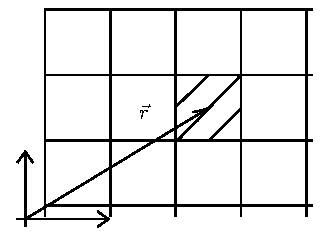
\includegraphics[width=0.5\textwidth]{../lessons/17_image/1.pdf}
\caption{\label{fig:17_1} Description.}
\end{figure}

\begin{equation}
  m_l (\va{r}) = \frac{1}{N_l} \sum_{i \in \va{r}}^{} S_i
\end{equation}
where \( N_l = (l/a)^D \) is the number of spins in each cell, if \( D \) is the dimension of the system.
\begin{remark}
This approach works if one assumes
\begin{equation}
  a \ll l \ll \xi (T) < L
  \label{eq:17_1}
\end{equation}
\end{remark}
\begin{remark}
Since close to \( T_c \) we have \( \xi \gg a \), we can always choose \( l \ll \xi  \) but still \( l \gg a \) such that the number \( N_l \) is large enough.
In this way, \( m(\va{r}) \) can be made to be a regular function of \( \va{r} \).
The little \( l \) cannot go to zero, because it is a physical quantity.
\end{remark}
\begin{remark}
In the reciprocal space (Fourier transform), bound \eqref{eq:17_1} implies the following cut off on the wave vector \( \va{q} \):
\begin{equation}
  \abs{\va{q}} > \Lambda  = l^{-1}
\end{equation}
No ultraviolet divergences can occur.
\end{remark}
We have
\begin{equation}
  Z = \sum_{m_l (\va{r})}^{} \qty(\sum_{\{ S^* \}  }^{} e^{-\beta \mathcal{H} ( \{ S \}  )}   )
 = \sum_{m_l(\va{r})}^{} e^{-\beta \mathcal{H}_{eff} [m(\va{r})]}
\end{equation}
If \( m(\va{r}) \) is regular, the sum converges to a functional integral
\begin{equation}
   Z_{GL} = \int_{}^{} \text{D}  \qty[m_l (\va{r})]  e^{-\beta \mathcal{H}_{eff}[m]}
\end{equation}
Let us now compute \( \mathcal{H}_{eff} [m] \).

\subsection{Computation of \( \mathcal{H}_{eff} [m]\)}
First let us notice that
\begin{equation}
  e^{-\beta \mathcal{H}_{eff} [m]} = \sum_{\{ S^* \}  }^{} e^{-\beta \mathcal{H}( \{ S \}  )}
\end{equation}
is proportional to the probability that the system displays a configuration with a profile \( m_l (\va{r}) \). \( \beta \mathcal{H}_{eff} [m] \) is made by two contributions:

\begin{enumerate}
\item Bulk contribution: terms relative to each cell.
We would expect that the hamiltonian will be very similar to the Landau. It is quite reasonable to say that in this case, \emph{inside}  a given cell \( l \ll \xi  \):
the boltzmann weight it is related to the exponent.

Since within each cell the system is uniform, we can consider the Landau free energy
\begin{equation}
  \beta \mathcal{H}_{eff}^b [m] = \bar{a} t m^2 + \frac{\bar{b} }{2} m^4
\end{equation}
\begin{equation}
  P^{cell} (m_l (\va{r})) \simeq \exp [ - \bar{a} t m^2 - \frac{b}{l} m^4 ]
\end{equation}
\item Surface term: term due to the interactions between adjiacant cells.
Let us consider a cell (Figure \ref{fig:17_2}, we can thing about different interactions.
\begin{figure}[h!]
\centering
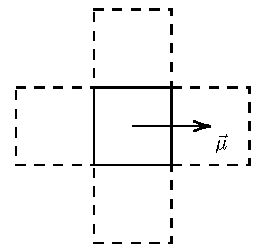
\includegraphics[width=0.3\textwidth]{../lessons/17_image/2.pdf}
\caption{\label{fig:17_2} Description.}
\end{figure}
We have \( \abs{\va{\mu }} =l  \), where \( \va{\mu } \) is a vector pointing towards the 2D neighbours. If we consider a simple quadratic interaction we can write
\begin{equation}
  - \beta \mathcal{H}_{eff}^s =   \sum_{\va{\mu }}^{}  \frac{\bar{K} }{2}\qty[ \qty(m_l (\va{r}+\va{\mu }) - m_l(\va{r}))^2] + O \qty[ \qty(m_l (\va{r}+\va{\mu }) - m_l(\va{r}))^4 ]
 \end{equation}
 \begin{remark}
  If \( l \) is small enough respect to \( \xi  \), we have other terms in this expansion \( (O[\dots]) \).
 \end{remark}
\end{enumerate}
The total energy is obtained  by summing over all the cells: is just given by the sum of the two term.
Now we have to sum over all the cell if we want to have the energy of the whole system.
We also look for the continuum limit:
\begin{equation}
  \sum_{\va{r}}^{}  \overset{\frac{l}{L} \ll 1}{\longrightarrow}   \frac{1}{l^D} \int_{}^{} \dd[D]{\va{r}}
\end{equation}
\begin{remark}
A lezione avevo scritto per \( \frac{l^D}{r} \ll 1 \), è la stessa cosa?????
\end{remark}
Let us consider the continuum limit for the
\begin{itemize}
\item Surface term.
\begin{equation}
\begin{split}
\frac{\bar{k} }{2} \sum_{\va{\mu }}^{} \sum_{\va{r}}^{}   \qty(m_l (\va{r}+\va{\mu }) - m_l(\va{r}))^2 &
\overset{\frac{l}{L} \ll 1}{\longrightarrow} \frac{\bar{k} }{2l^{D-2}} \sum_{\va{\mu }}^{} \int_{}^{} \dd[D]{\va{r}} \qty(\frac{m_l (\va{r}+\va{\mu }) - m_l(\va{r})}{l})^2 \\
& = \frac{\bar{k} }{2l^{D-2}} \int_{}^{} \dd[D]{\va{r}} \sum_{\va{\mu }}^{}  \qty(\frac{m_l (\va{r}+\va{\mu }) - m_l(\va{r})}{l})^2 \\
& \overset{\frac{a}{L} \ll \frac{l}{L} \ll 1}{\simeq } \int_{}^{} \frac{\bar{k} }{2l^{D-2}}  \sum_{\va{\mu }}^{} \qty(\pdv{m_l}{\chi _ \mu } )^2   \dd[D]{\va{r}} \\
& \overset{\frac{a}{L} \ll \frac{l}{L} \ll 1}{ \longrightarrow }
\int_{}^{} \dd[D]{\va{r}} \frac{k}{2} \qty(\bar{\grad } m_l (\va{r}) )^2
\end{split}
\end{equation}
where
\begin{equation}
  k \equiv  \frac{ \bar{k} }{l^{D-2}}
\end{equation}
so rescaling the elastic constant by \( l^{D-2} \). In this way the result is indipendent on \( l \).

\item Bulk term.
We have
\begin{equation}
  \sum_{\va{r}}^{} -\bar{a}  t m^2 (\va{r}) \overset{\frac{l}{L} \ll 1}{\longrightarrow}   \frac{1}{l^D} \int_{}^{} -  \bar{a}   t m^2 (\va{r}) \dd[D]{\va{r}}= \int_{}^{} -  a t m^2 (\va{r}) \dd[D]{\va{r}}
\end{equation}
with
\begin{equation}
  a \equiv \frac{\bar{a} }{l^D}
\end{equation}
Similarly we have
\begin{equation}
  b \equiv \frac{\bar{b} }{l^D}
\end{equation}
Consider
\begin{equation}
  \beta \mathcal{H}_{eff} [m] = \int_{}^{} \dd[D]{\va{r}} \qty[a t m^2 (\va{r}) + \frac{b}{2} m^4 (\va{r}) + \frac{k}{2} (\bar{\grad } m (\va{r}))^2]
\end{equation}
\begin{equation}
  Z_{GL} = \int_{}^{} \text{D}\qty[m(\va{r})]   e^{-\beta \mathcal{H}_{eff}}
\end{equation}
\end{itemize}
Some considerations:
\begin{enumerate}
\item If \( m(\va{r}) = m \) (uniform system) we go back to the Landau theory.
\item For non uniform system there is a new term given by \( \qty(\va{\grad } m (\va{r})^2 ) \). This term can be also added directly to the Landau theory by simply assuming that, whe \( m \rightarrow m(\va{r}) \), one has to consider an additioned energy cost due to small variation of \( m \).
\end{enumerate}
Why we take \( \qty(\va{\grad }m)^2  \) and not something else?
The choise is first of all a consequence of the isotropy of the system (all directions are equivalent).
Among all the possible combinations of partial derivatives that are invariant by spatial rotations the term, \( \qty(\va{\grad }m)^2  \) is the simplest one.
\begin{remark}
When \( m \rightarrow \va{m} \) (\( O(n) \) models) we have
\begin{equation}
  (\grad \va{m})^2 = \sum_{i=1}^{n} \sum_{\alpha =1}^{D} \sum_{\beta =1}^{D} \partial_ \alpha {m_i} \partial_ \beta  {m_i}
\end{equation}
Higher order terms are
\begin{equation}
  \qty(\grad ^2 \va{m})^2 =  \sum_{i=1}^{n} \sum_{\alpha =1}^{D} \sum_{\beta =1}^{D}
  \qty(\partial_ \alpha \partial_ \alpha {m_i}) \qty( \partial_ \beta \partial_ \beta {m_i})
\end{equation}
and
\begin{equation}
  \va{m}^2 \qty(\grad  \va{m})^2 =  \sum_{i=1}^{n} \sum_{j=1}^{n} \sum_{\alpha  =1}^{D} m_i m_i \partial_ \alpha {m_j} \partial_ \alpha {m_j}
\end{equation}
In most cases it is sufficient to consider only the lowest order term.
\end{remark}
\subsection{Magnetic non homogeneous field}
\begin{equation}
  \va{h} ( \va{r}) \equiv \beta \va{H} ( \va{r})
\end{equation}
Additional term (Legendre transform)
\begin{equation}
  - \int_{}^{} \dd[D]{\va{r}} \va{h} (\va{r}) \vdot \va{m} (\va{r})
\end{equation}
Going back to the scalar case, the usual partition function is
\begin{equation}
  Z_{GL}^h = \int_{}^{} \text{D} [m(\va{r})] e^{  -\int_{}^{} \dd[D]{\va{r}} \qty[a t m^2 (\va{r}) + \frac{b}{2} m^4 (\va{r}) + \frac{k}{2} (\bar{\grad } m (\va{r}))^2 - h(\va{r})m(\va{r}) ]  }
\end{equation}
and we define
\begin{equation}
  F_{eff}[m] = -\int_{}^{} \dd[D]{\va{r}} \qty[a t m^2 (\va{r}) + \frac{b}{2} m^4 (\va{r}) + \frac{k}{2} (\bar{\grad } m (\va{r}))^2 - h(\va{r})m(\va{r})]
\end{equation}
\subsubsection{Functional derivatives}
\begin{equation}
  \frac{\delta G(h (\va{r}))}{\delta h (\va{r})} \equiv  \lim_{\varepsilon \rightarrow 0} \frac{G(h[\va{r}+G])- G(h[\va{r}])}{\varepsilon }
\end{equation}
\begin{example}{}{}
\begin{equation}
  \frac{\delta f (\va{r}')}{\delta f (\va{r})} = \delta ^D (\va{r}' - \va{r})
\end{equation}
\begin{equation}
  \frac{\delta }{\delta m (\va{r})} \qty[ \int_{}^{} \dd[D]{\va{r}'} \frac{k}{2} \qty(\grad m (\va{r}'))^2     ]  \overset{to do}{=} - k \grad ^2 m
\end{equation}
\end{example}
where
\begin{equation}
  \delta G [ \grad m] = \qty[ \int_{}^{} \dd[D]{\va{r}'} \frac{k}{2} ( \grad m(\va{r}))^2  ]
\end{equation}
\begin{equation}
  \delta G = G \qty[ \grad [m+\delta m]] - G [\grad m]
\end{equation}
The average is
\begin{equation}
  \expval{m(\va{r})} = - \frac{\delta F}{\delta h (\va{r})} = - \frac{\delta \ln{Z[h]} }{\delta h (\va{r})}
\end{equation}
and one can show that the magnetic suscpetibility is
\begin{equation}
\begin{split}
  \chi  (\va{r},\va{r}') & = \frac{\delta ^2 F}{\delta h(\va{r}) \delta h(\va{r}')}
  = \beta ^{-1} \frac{\delta ^2 \ln{Z[h]} }{\delta h (\va{r}) \delta h (\va{r}')}\\
  & = \beta ^{-1} \qty[ \expval{m(\va{r}) m (\va{r}')} - \expval{m (\va{r})} \expval{m(\va{r}')}  ] \\
  & = \beta ^{-1} G_c (\va{r},\va{r}') \\
\end{split}
\end{equation}
The problem is again try to approximate this term as much as we can.
Let us compute the approximation.






\section{Saddle point approximation and Landau theory for non-homogeneous systems}
\begin{equation}
  Z_{GL}[h] = \int_{}^{} \text{D} [m] e^{- \int_{}^{} \dd[D]{\va{r}} \qty[\beta \mathcal{H}_{eff} [m] - h (\va{r}) m (\va{r})]   }
\end{equation}
where \( h(\va{r}) = \beta H(\va{r}) \) and
\begin{equation}
  \beta \mathcal{H}_{eff} [m] = a t m^2 + \frac{b}{2} m^4 + \frac{k}{2} \qty(\grad m)^2
\end{equation}
We noe approximate the functional integral with its dominant term, i.e. with the one for which the exponent
\begin{equation}
  L (m,h) = \int_{}^{} \dd[D]{\va{r}}  \qty[\beta \mathcal{H}_{eff} - h m]
\end{equation}
is minimum. Let \( m_0 (\va{r}) \) be the profile for which \( L (m_0 (\va{r}), h (\va{r}) ) \) is minimum. It implies
\begin{equation}
  Z_{GL} [h] \overset{\substack{ \text{Saddle} \\  \text{point} } }{\simeq } Z_{GL}^0 [h] = e^{- L [m_0]}
\end{equation}
In order to find the minimum, one has to consider the stationarity condition
\begin{equation}
  \delta L = 0
  \label{eq:17_3}
\end{equation}
where
\begin{equation}
  L [m,h] = \int_{}^{} \dd[D]{\va{r}} \qty[\beta \mathcal{H}_{eff} [m] - h m]
\end{equation}
By considering \( \delta L \) with respect to the variations \( \delta m \) and \( \delta (\grad m) \) one gets the equation of state
\begin{equation}
  h (\va{r}) = - \qty[\grad \qty(\pdv{ \mathcal{H}_{eff}}{(\grad m)} ) - \pdv{\mathcal{H}_{eff}}{m}  ]
  \label{eq:17_2}
\end{equation}
  \begin{remark}
  For \( h=0 \), equation \eqref{eq:17_2} reduces to the Euler-Lagrande equation
  \begin{equation}
    \pdv{\mathcal{H}_{eff}}{m} = \grad \qty(  \pdv{\mathcal{H}_{eff}}{(\grad m)})
  \end{equation}
  \end{remark}
Indeed, let
\begin{equation}
  L [m, \grad m,h] = \int_{}^{} \dd[D]{\va{r}} \mathcal{L} (m, \grad m,h)
\end{equation}
Let us consider \( h=0 \) and look for the variation of \( L \) with respect to the variations of \( m,\, \delta m \)  and the variation of \( \grad m, \, \delta (\grad m) \),\begin{equation}
\begin{split}
\delta L [m, \grad m,0]  &=  \int_{}^{} \dd[D]{\va{r}} \mathcal{L} (m+\delta m, \grad m + \delta (\grad m)) - \int_{}^{} \dd[D]{\va{r}} \mathcal{L} (m,\grad m)    \\
& = \int_{}^{} \dd[D]{\va{r}} \qty[\mathcal{L} (m+\delta m, \grad m + \delta ( \grad m)) - \mathcal{L} (m, \grad m)] \\
& = \int_{}^{} \dd[D]{\va{r}} \qty[\pdv{\mathcal{L}}{m} \delta m + \underset{f}{\pdv{\mathcal{L}}{(\grad m)} } \underset{g'}{\delta (\grad m) }  ]
\end{split}
\end{equation}
We now integrate by parts the second term
\begin{equation}
\delta L = \int_{}^{} \dd[D]{\va{r}} \qty[\pdv{\mathcal{L}}{m} \delta m - \grad  \pdv{\mathcal{L}}{(\grad m)} \delta m ] + \underbrace{\int_{V}^{} \dd[D]{\va{r}} \grad \qty[\pdv{\mathcal{L}}{\grad m} \delta m ] }_{}
\end{equation}
Reming the divergence theorem \( \int_{\partial{ \Omega }}^{} F = \int_{V}^{} \grad F     \), the second term vanishes at the boundary of the integration.
\begin{equation}
  \delta L = \int_{}^{} \dd[D]{\va{r}} \qty[\pdv{\mathcal{L}}{m} - \grad \pdv{\mathcal{L}}{(\grad m)}  ] \delta m
\end{equation}
Remind the stationarity condition \eqref{eq:17_3}, \( \forall \delta m \neq 0 \), if and only if  the Euler-Lagrange equation
\begin{equation}
  \pdv{\mathcal{L}}{m} - \grad \qty(\pdv{\mathcal{L}}{(\grad m)} ) = 0
\end{equation}
In our case, when \( h=0 \) we have \( \mathcal{L} \rightarrow \beta \mathcal{H}_{eff} \). Since
\begin{equation}
  \beta \mathcal{H}_{eff} = a t m^2 + \frac{b}{2} m^4 + \frac{k}{2} (\grad m)^2
\end{equation}
the Euler-Lagrange equation become
\begin{equation}
  h (\va{r}) = - k \grad ^2 m_0 (\va{r}) + 2 a t m _0 (\va{r}) + 2 b m_0^3 (\va{r})
   \label{eq:17_4}
\end{equation}
this is the mean field solution of the Gibbs-Landau. It is more general than the Landau we have used. It is just the Landau with the additional term \( \grad  \).
\begin{remark}
If \( h (\va{r}) = h \) (homogeneous field) and \( m_0 (\va{r})=m_0 \), equation reduces to the equation of state of the Landau theory of uniform system
\begin{equation}
  h = 2 a t m_0 + 2 b m_0 ^3
\end{equation}
 \end{remark}
 \begin{remark}
 A mean field theory of systems with spatial disomogeneity can start directly by considering the free energy functional
 \begin{equation}
   F[m,h] = \int_{}^{} \dd[D]{\va{r}} \qty[a t m^2 (\va{r}) + \frac{b}{2} m^4 (\va{r}) + \frac{k}{2} (\grad m)^2 - h (\va{r}) m(\va{r})]
 \end{equation}
 \end{remark}

 \subsubsection{lesson}
 \begin{equation}
 Z_{GL}^h = \int_{}^{} \text{D}[m] \exp (-F_{eff}[m])
 \end{equation}

 In the frist approximation, we replace this integral with just
 \begin{equation}
   \simeq \exp [-\beta F_{eff} [\bar{m} ] ]
 \end{equation}
 where \( \bar{m}(\va{r})  \) is such that \( F_{eff} [\bar{m} ] \) is minimal.
 \begin{equation}
   \bar{m} =  \min_{m} [F_{eff}[m]]
 \end{equation}
 Taking the variation of \( \delta F_{eff} \) when \( m \rightarrow m + \delta m \):
 \begin{equation}
   \delta F_{eff} = F_{eff} [m+\delta m] - F_{eff} [m]
 \end{equation}
 \begin{equation}
   h (\va{r}) = - \qty[\grad \qty(\pdv{ \mathcal{H}_{eff}}{(\grad m)} ) - \pdv{\mathcal{H}_{eff}}{m}  ]
 \end{equation}




\section{Nono homogeneous systems and correlation functions within a mean field approximation}
Let us now try to compute the correlation function. Starting from \eqref{eq:17_4}, we derive it (is a functional derivative!) with respect to \( h (\va{r}')\).

Remembering that
\begin{equation}
  \chi _T (\va{r},\va{r}') = \frac{\delta m(\va{r})}{\delta h (\va{r}')}
\end{equation}
and
\begin{equation}
  \frac{\delta h (\va{r})}{\delta h (\va{r}')} = \delta (\va{r}-\va{r}')
\end{equation}
we have
\begin{equation}
  \delta  (\va{r} - \va{r}')  = \qty[- k \grad ^2 + 2 a t    + 6 b m_0^2 (\va{r}) ] \chi _T (\va{r}-\va{r}')
\end{equation}
where we have assumed translational invariance.

On the other hand, from fluctuation dissipation relation
\begin{equation}
  G_c (\va{r}-\va{r}') = k_B T \chi _T (\va{r}-\va{r}')
\end{equation}
we obtain
\begin{equation}
  \beta \qty[-k \grad ^2 + 2 a t + 6 b m_0 ^2 ] G_c (\va{r}-\va{r}') = \delta (\va{r}- \va{r}')
  \label{eq:17_5}
\end{equation}
The equation \eqref{eq:17_5} is also known as fundamental equation and \( G_c (\va{r}- \va{r}') \)  the fundamental solution or green function of the differential operator
\begin{equation}
  D \equiv - k \grad ^2 + 2 a t + 6 b m^2
\end{equation}
We now look for the solutions of \eqref{eq:17_5}.  We consider two cases, \( T > T_c \) and \( T < T_c \) and let \( h \rightarrow 0 \).
\begin{itemize}
\item Case \( T > T_c \) \( (t>0) \) : the mean field solution is \( m_0 (\va{r}) = m_0 = 0 \). Hence,
\begin{equation}
  \qty(-k \grad ^2 + 2 a t ) G_c (\va{r}-\va{r}') = k_B T \delta (\va{r}-\va{r}')
  \label{eq:17_6}
\end{equation}
By calling
\begin{equation}
  \xi_> (t) = \qty(\frac{k}{2 a t })^{1/2}
\end{equation}
we have
\begin{equation}
  \qty(-\grad ^2 + \xi _> ^{-2} (t)) G_c (\va{r}-\va{r}') = \frac{k_B T}{k} \delta (\va{r}-\va{r}')
\end{equation}
\item Case \( T < T_c \) \( (t<0) \). Let us conside the omogeneous solution
\begin{equation}
  m_0 = \pm \qty(-\frac{at}{b})^{1/2}
\end{equation}
This gives
\begin{equation}
  \qty(-\grad ^2 + \xi _<^{-2} (t))G_c (\va{r}- \va{r}') = \frac{k_B T}{k} \delta (\va{r}- \va{r}')
\end{equation}
where
\begin{equation}
  \xi _{<} (t) = \qty(- \frac{k}{4at})^{1/2}
\end{equation}
\end{itemize}
\begin{remark}
In both cases \( \xi \sim t^{-1/2} \), we have \( \nu = \nu ' = \frac{1}{2} \), that is the mean field value of \( \nu  \)!
\end{remark}
\begin{remark}
Since \( \nu = 1/2 \), the upper critical dimension of a critical point belonging to the Ising universality class is
\begin{equation}
  D_c = \frac{2}{\nu } = 4
\end{equation}
\end{remark}
For both cases, the equation for \( G_c (\va{r}-\va{r}') \) has the following form
\begin{equation}
  \qty(- \grad ^2 + \xi ^{-2}) G_c (\va{r}-\va{r}') = \frac{k_B T}{k} \delta (\va{r}-\va{r}')
\end{equation}

This equation can be solved in at least two ways:
\begin{itemize}
\item Fourier transform.
\item Spherical coordinates.
\end{itemize}







\end{document}
